\subsection{桥接模式(Bridge)}

\subsubsection{桥接模式简介}

桥接模式(Bridge Pattern)是一种结构型设计模式,它将抽象部分与它的实现部分分离,使它们都可以独立地变化。这种模式提供了一种将抽象部分与实现部分分离的方法,从而使得它们可以独立地变化。它是用组合关系代替继承关系来实现,从而降低了抽象和实现这两个可变维度的耦合度。

\subsubsection{桥接模式在项目中的应用}

\begin{figure}[h]
  \centering
  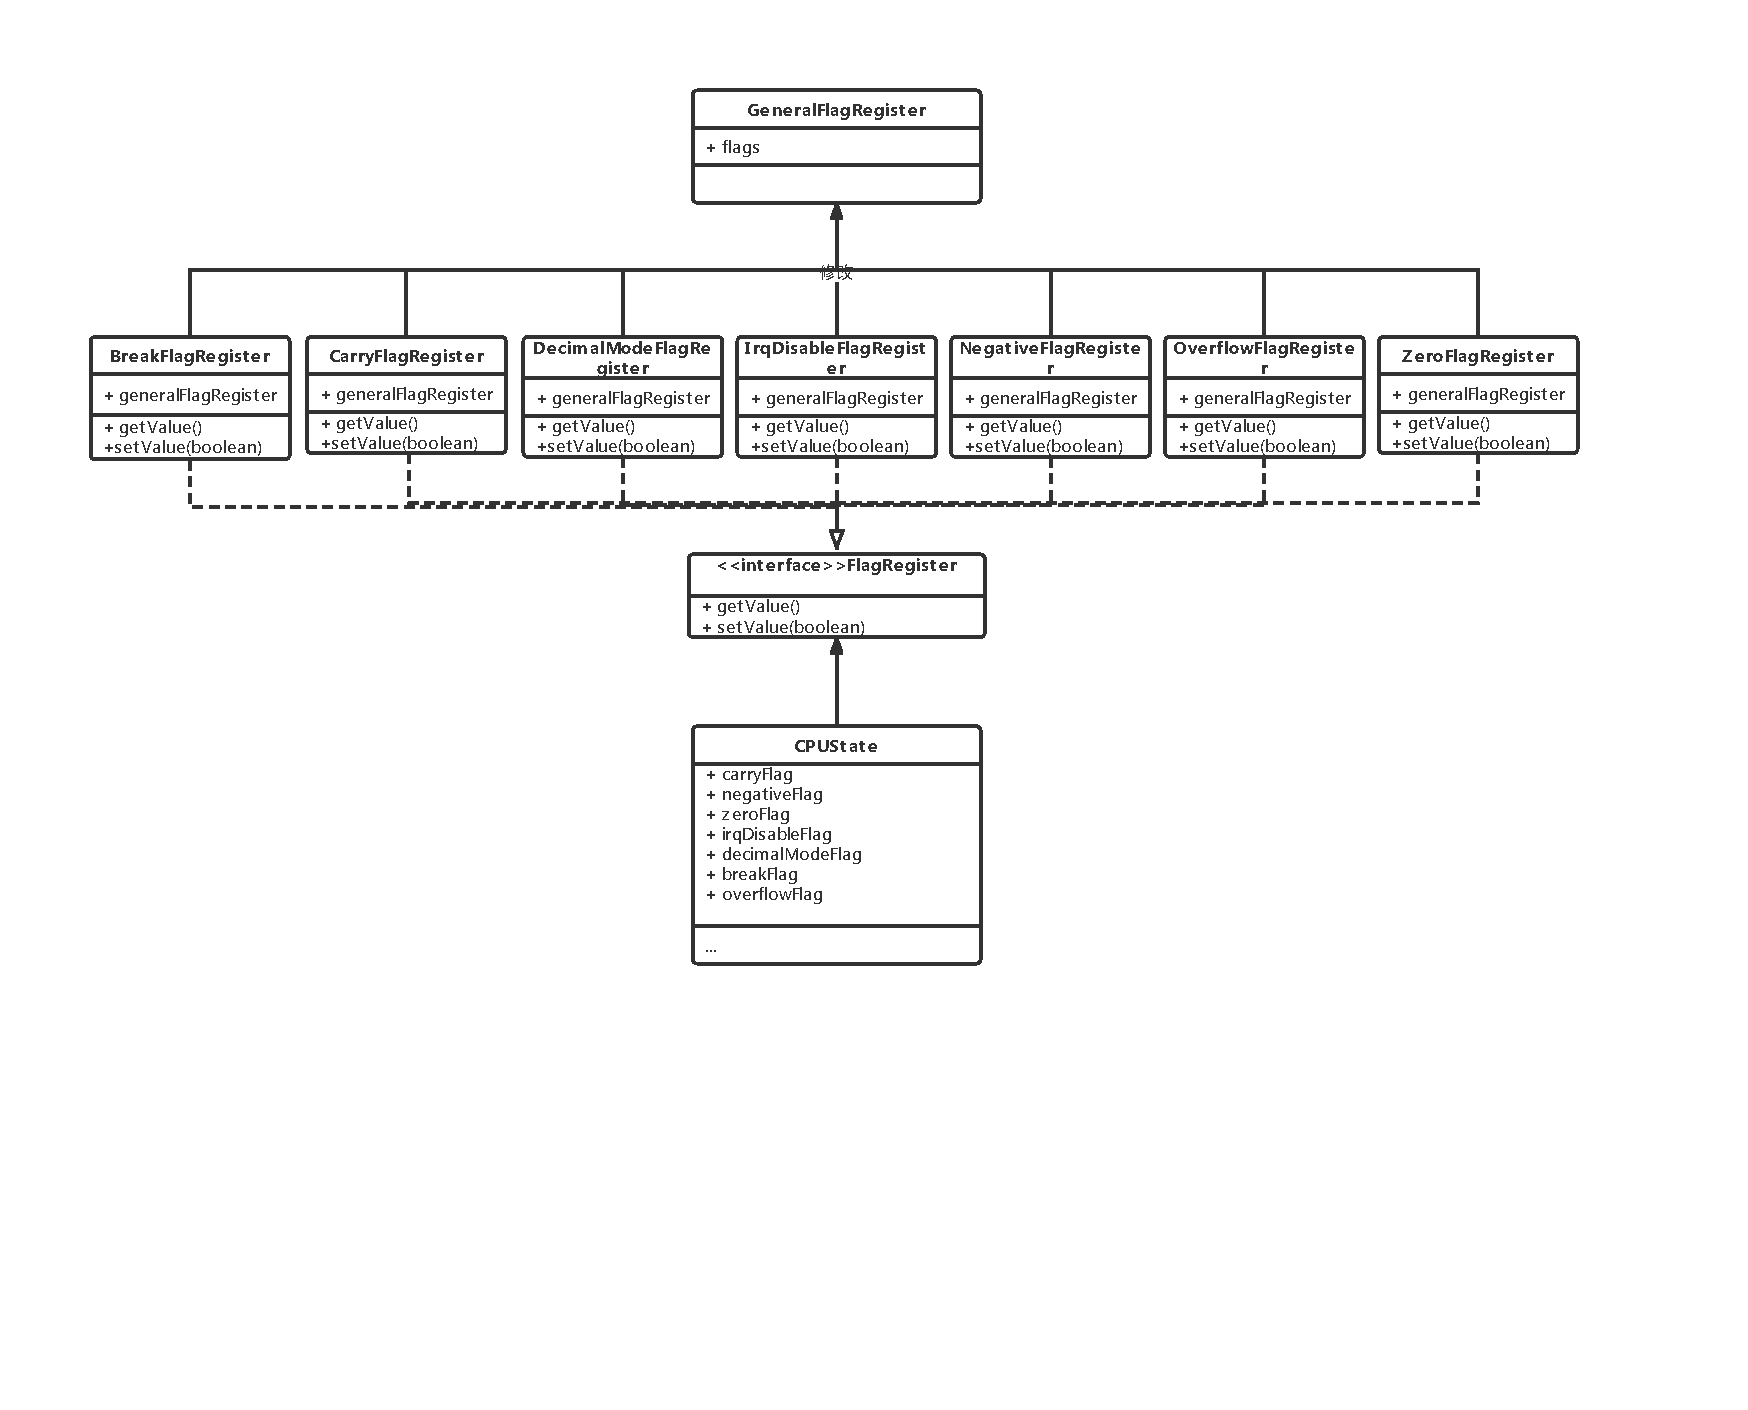
\includegraphics[width=0.9\textwidth]{figures/Bridge.pdf}
  \caption{桥接模式在 Slow6502 中的类图}
\end{figure}

在我们的项目中,我们使用桥接模式包装对状态寄存器各个位的访问。使用桥接模式包装对状态寄存器各个位的访问可以有效地分离抽象部分(对状态寄存器各个位的访问)与实现部分(状态寄存器的存储)。

这样设计的好处在于,可以使得抽象部分和实现部分可以独立地变化。例如,如果你需要更改 MOS 6502 模拟器中状态寄存器的存储方式,可以只修改实现部分的代码,而不需要更改对状态寄存器各个位的访问的代码。这样,你就可以更加高效地开发和维护 MOS 6502 模拟器。

另外,使用桥接模式还可以使得 MOS 6502 模拟器的设计更加模块化,更易于复用。例如,如果你需要在其他项目中使用 MOS 6502 模拟器中实现的对状态寄存器各个位的访问功能,你可以将这部分功能抽象为接口,然后在其他项目中直接调用这个接口,而无需拷贝代码。这样,你就可以在不同项目中复用 MOS 6502 模拟器中的代码,提高开发效率。
